\newcommand{\posterAsymmetry}[2]{

\setlength{\frameWidth}{#1}
\setlength{\frameHeight}{#2}
\setlength{\unitlength}{0.02\frameWidth}
\psset{unit=\unitlength}

\rput[tr](49,30){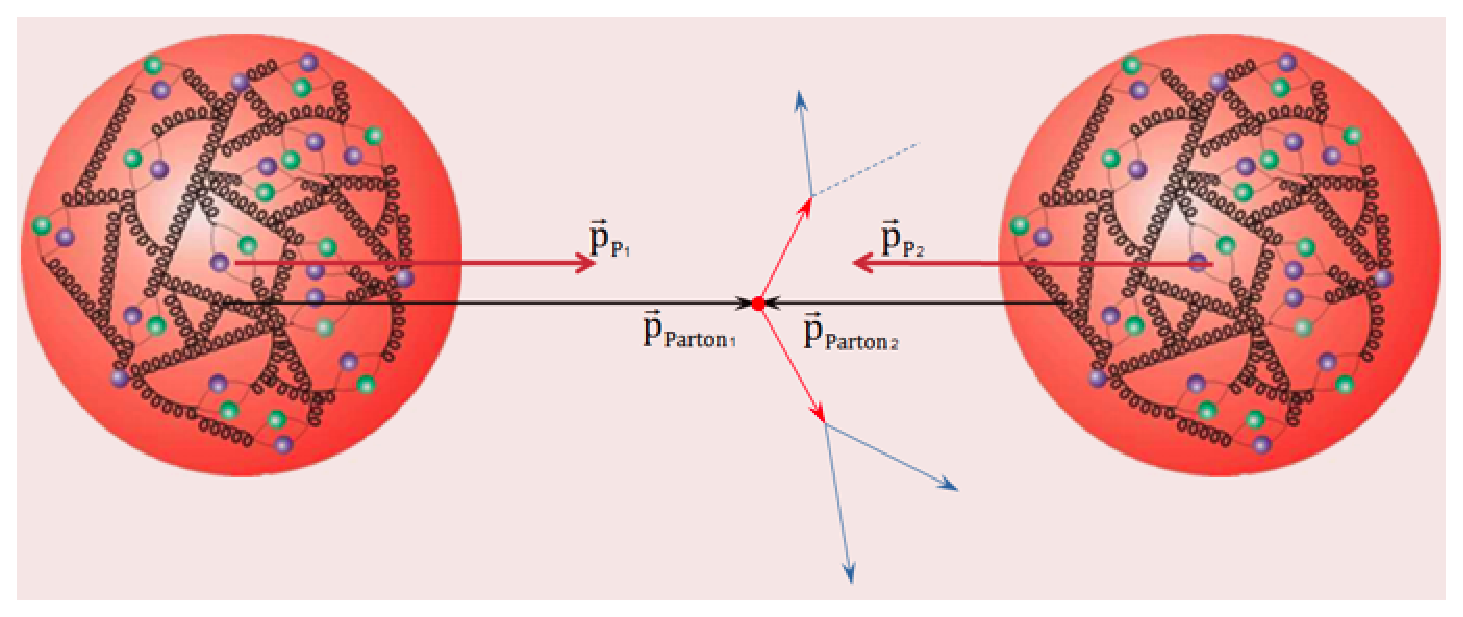
\includegraphics[width=29\unitlength]{graphics/proton_coll3}}

\rput[lt](2,27) {%
\begin{minipage}{20\unitlength}

\raggedright

\begin{list}{\labelitemi}{\setlength{\itemsep}{0mm}
                          \setlength{\topsep}{0mm}
                          \setlength{\leftmargin}{0mm}
                          \setlength{\rightmargin}{0mm}}

   \item Due to spin the product of proton collisions can have spacial asymmetry w.r.t. the spin direction

\end{list}

\end{minipage}
}


\rput[lt](2,16) {%
\begin{minipage}{49\unitlength}

\raggedright

\begin{list}{\labelitemi}{\setlength{\itemsep}{-3mm}
                          \setlength{\topsep}{0mm}
                          \setlength{\leftmargin}{0mm}
                          \setlength{\rightmargin}{0mm}}

   \item The knowledge about the internal proton structure is extracted from the measured asymmetry:
   %
   \vspace{-0.8\unitlength}
   \begin{equation*}
   \underbracket{A = \frac{1}{P} \times \frac{N^{\uparrow} - N^{\downarrow}}{N^{\uparrow} + N^{\downarrow} }}_{\text{\normalsize single spin asymmetry}}
   \hspace{8\unitlength}
   \underbracket{\mathbb{A} = \frac{1}{P^2} \times \frac{N^{\uparrow\uparrow} - N^{\uparrow\downarrow}}{N^{\uparrow\uparrow} + N^{\uparrow\downarrow} }}_{\text{\normalsize double spin asymmetry}}
   \end{equation*}

   \vspace{-0.8\unitlength}

   \item We must know the spin direction of colliding protons (only at RHIC!)

   \item \textbf{Precise knowledge of polarization \boldmath $P \pm \Delta P$ is essential for all spin analyses at RHIC}

\end{list}

\end{minipage}
}


%\rput{0}{\psgrid[gridlabels=0.7,subgriddiv=0, griddots=3](1,-1)(0,0)(\myPsPictureWidthLocal,\myPsPictureHeightLocal)}

}

\setlength{\unitlength}{10mm}
\psset{unit=\unitlength}
